\section{Simulations}\label{sec:simulation}

The ODE (Open Dynamics Engine) library \cite{ode:2008} is used to test the iterative mass displacement compensation algorithm presented in the previous section. The initial position of the hopping quadruped robot is shown in Fig \ref{fig:ODESimulations}a. Each leg is composed of two spring-damper joints, the first one being passive and connects the red and green cylinder together; and the second, active one, connects the green cylinder with the robot body. The body consists of 4 joined masses indexed as 1 (white), 2 (red), 3 (green) and 4 (blue). All the parameters of the  robot simulation are shown in \ref{tab:RobotDimensions}.

\begin{table}
\centering
\begin{tabular}{|c|c|}
	\hline
	$Body\: size$ &  $[0.30\: 0.15\: 0.01]m$ \\
	\hline
	$Lower\:leg\:size$ &  $0.05m$ \\
	\hline
	$Upper\:leg\:size$ &  $0.05m$ \\
	\hline
	$Leg\:radius$ &  $0.01m$ \\
	\hline
	$Total\:leg\:mass$ &  $0.15kg$ \\
	\hline
	$Passive\:spring\:constant/damping$ &  $2000N/m, 50Ns/m$ \\
	\hline
	$Active\:spring\:constant/damping$ &  $10000N/m, 30Ns/m$ \\
	\hline
	$Tail\:length$ &  $0.1m$ \\
	\hline
	$Tail\:radius$ &  $0.005m$ \\
	\hline
\end{tabular}
\caption{Robot simulation parameters}\label{tab:RobotDimensions}
\end{table}



The active springs generates forces periodically with the period interval $Td=1s$ which accelerate the body and produce rotational vector which is recorded during the acceleration phase. The applied spring force is minimal, but sufficient enough to produce measurable angular speed and to keep the time needed to calm the body oscillations down to a minimum. The acceleration phase lasts for about 200ms after which the body calms in the next 800ms. The initial tail angles are $q_1=0$ and $q_2=0$ as illustrated in Fig. \ref{fig:ODESimulations}a.

\begin{table}
	\centering
\begin{tabular}{|c|c|c|c|c|}
	\hline
$Test$ &  $Mass[kg]$ & $q$  & $\left \| \vec{\boldsymbol{\omega}} \right \|$ & $K_0$\\
	\hline
0   & $[0\: 0\: 1\: 1]$ & $[89.99\: 32.86]$ & 0.0026 & 0.3\\
1   & $[1\: 1\: 0\: 0]$ & $[-89.99\: 32.20]$ & 0.0038 & 0.3\\
2   & $[1\: 1\: 1\: 0]$ & $[-25.43\: 29.15]$ &  0.003 & 0.3\\
3   & $[1\: 1\: 1\: 0]$ & $[-23.26\: 29.20]$ &  0.003 & 0.6\\
\hline
\end{tabular}
\caption{Testing parameters}\label{tab:Simulations}
\end{table}



\begin{figure}
	\centering
	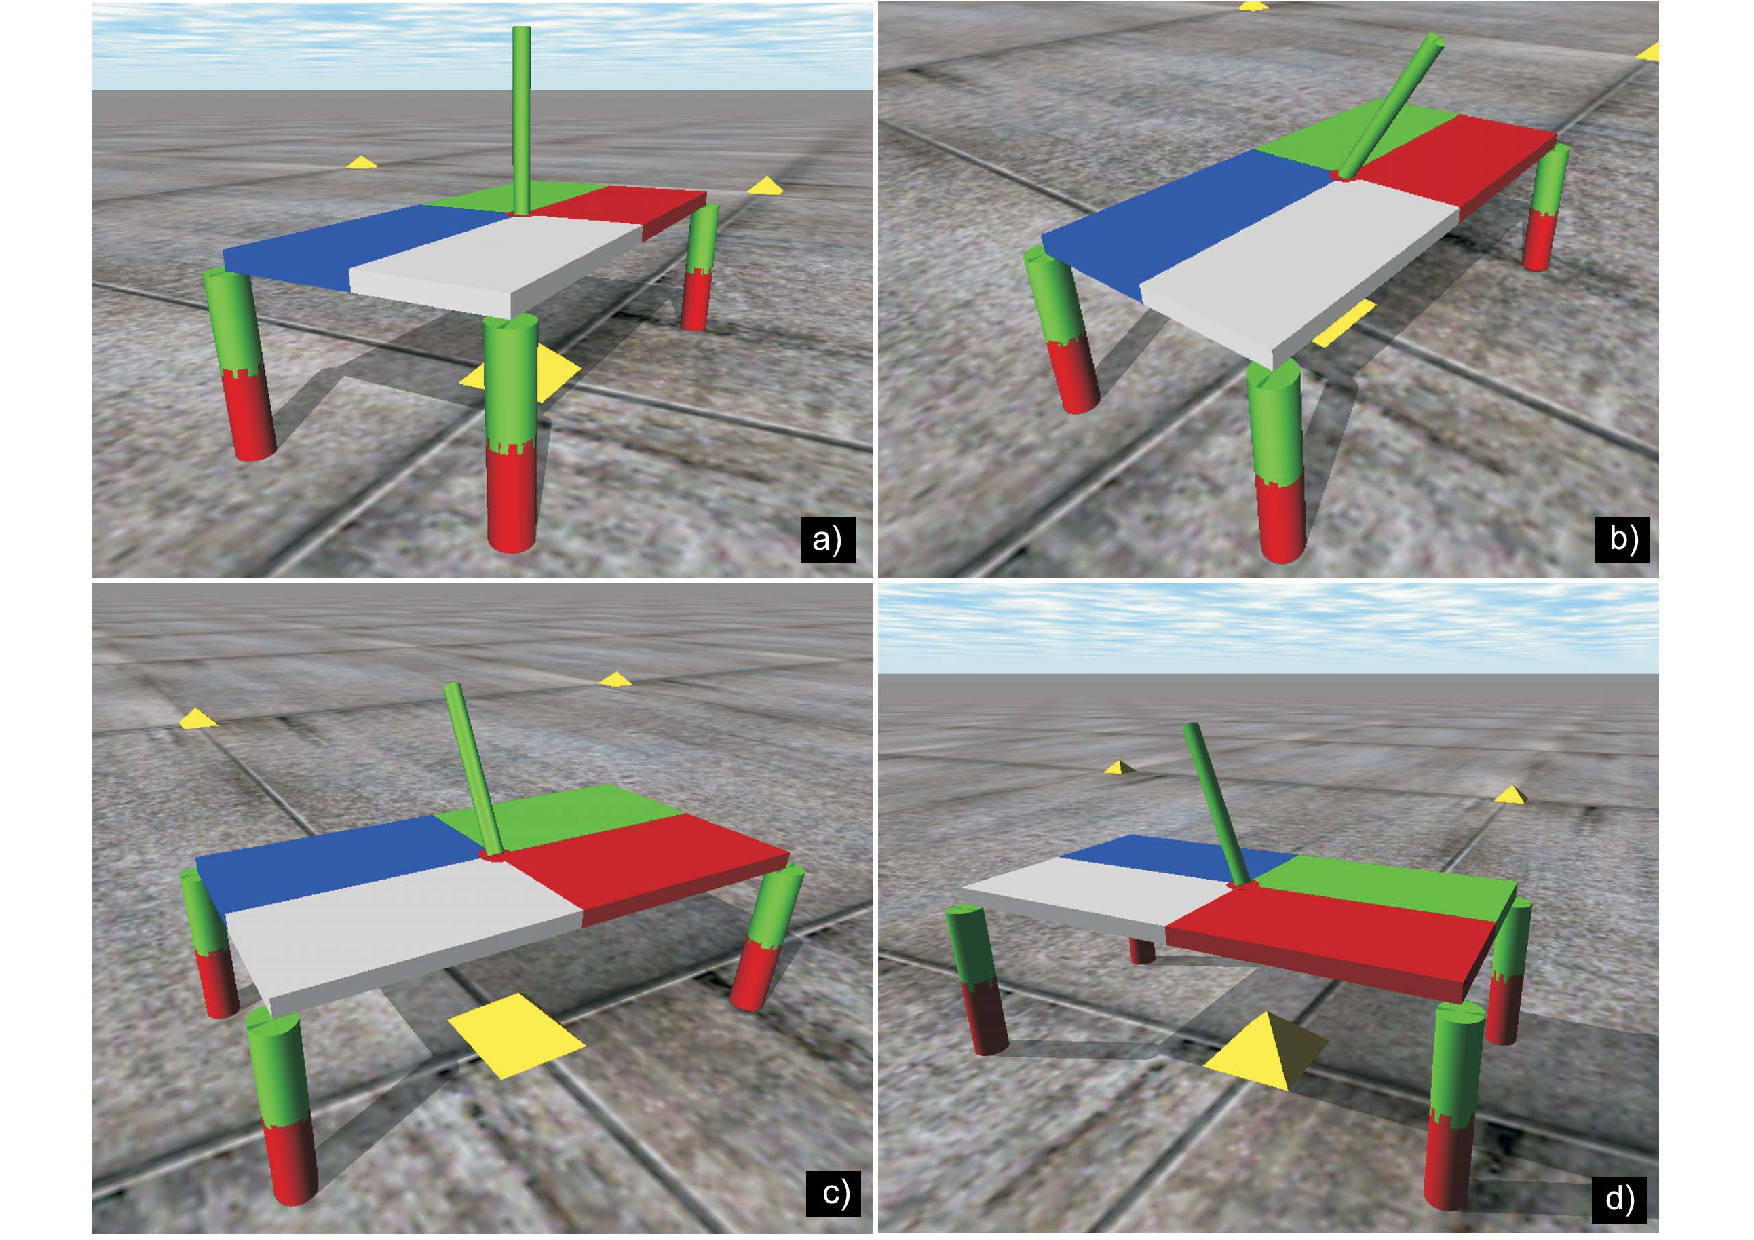
\includegraphics[width=80mm]{./pictures/ODE_simulations.pdf}
	\caption{ODE simulations. a) Initial position b) Test 1. c) Test 2. d) Test 3.}
	\label{fig:ODESimulations}
\end{figure}

For this paper, a series of four experiments is conducted by varying the initial mass distribution of the robot, as shown in Table \ref{tab:Simulations}. The first column represents body mass redistribution vector, while the second and the third are the final results of tail angles and angular rotation values, respectively. The simulation results are presented in Fig. \ref{fig:ODE graph}. 

Test 1: For a negligibly small masses of white and red cuboids, the algorithm consequently titled tail in the direction $q1=90^{\circ}$. The tail reaches the desired position in 7-10 seconds and the final inclination is $q2=32.86^{\circ}$(Fig. \ref{fig:ODESimulations}b). The angular velocity value $\left \| \vec{\boldsymbol{\omega}} \right \|$ falls from $0.14$ to final $0.0025$.

Test 2: When the green and blue cuboid masses are negligible, the algorithm tilts the tail in the direction $q1=-90^{\circ}$. The final tail inclination is $q2=32.20^{\circ}$(Fig. \ref{fig:ODESimulations}b). The angular velocity value $\left \| \vec{\boldsymbol{\omega}} \right \|$ goes from $0.14$ to final $0.0038$. 

Test 3: When only the blue cuboid mass is negligible, the algorithm tilts the tail in the direction $q1=-25.43^{\circ}$. The final tail inclination is $q2=29.15^{\circ}$(Fig. \ref{fig:ODESimulations}c). The algorithm requires a longer time to minimize $\left \| \vec{\boldsymbol{\omega}} \right \|$ to final $0.0025$(see Table \ref{tab:Simulations2}).

Test 4: This experiment was conducted with the same initial parameters as in Test 3, except this time the higher gain $K_0$ was used. The desired position is reached faster as expected. The subsequent increase has shown to cause small oscillations in the result. By comparing Fig. 5, it is interesting to notice how joint angle $q_1$ takes more time to achieve the desired equilibrium. This is obvious, since according to Fig 5, once the algorithm reaches the saddle of equation (22), the slope in $q_1$ direction is very small.

\begin{table}
	\centering
\begin{tabular}{|c|c|c|c|}
	\hline
$Interation$ & $q_1$ & $q_1$  & $\left \| \vec{\boldsymbol{\omega}} \right \|$\\
	\hline
1 & -53.71 & 10.19 & 0.060\\
5 & -36.89 & 21.75 & 0.012\\
10 & -32.44 & 27.03 &  0.005\\
15 & -29.09 & 28.81 & 0.004\\
20 & -25.43 & 29.15 &  0.003\\
\hline
\end{tabular}
\caption{Test 3. results}\label{tab:Simulations2}
\end{table}

\begin{figure}
	\centering
	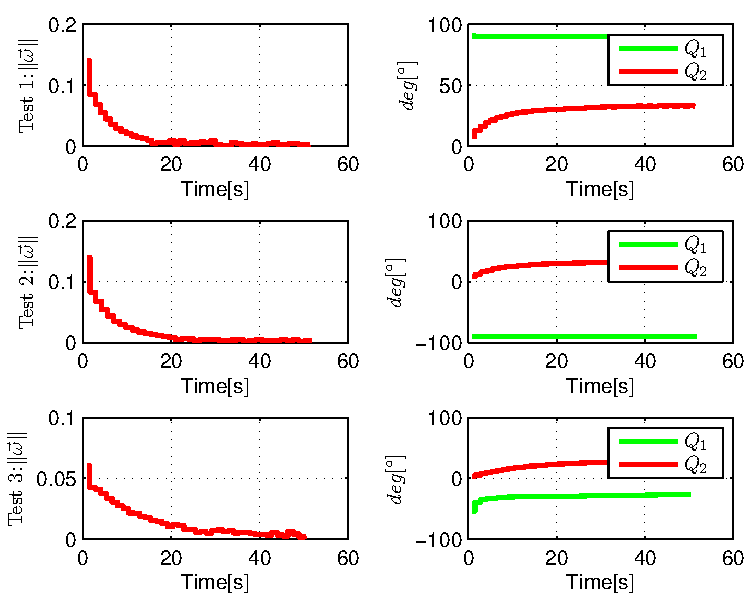
\includegraphics[width=90mm]{./pictures/ODE_graph.pdf}
	\caption{ODE simulations, Test 1-4.}
	\label{fig:ODE graph}
\end{figure}


